\chapter{Problem and State of the Art}

\section{Problem}

The Lightning Network protocol as described in \ref{sec:lightning_network} is 
driven by a consensius between group of implementors in order to standardize
a feature. Where most of the time in order to adress a well known problem a data 
driven analysis on a groupd of nodes it is required in order to emphasize the
problem and sometimes also to see the real impact of the solution after be 
implemented but before begin a standard.
However, in order to perform a data driven analysis in an ecosystem where the decision
is drive by a kind of consensius, it is required also to some kind of 
constraint on how this data driven analysis is perform and analyzed across 
different implementations.

\subsection{Data Drive Analysis on the Lightning Network}

Currently the most common data driven analysis on the Lightning Network is performed 
on gossip data where any node can with at least one public channel can 
have access to. An example of this kind analysis is descrived in \cite{lngossip}
where the data are collected from core lightning and archived.

However, at the current state of the art there is no example on how to perform
an data driven analysis on local data collected across implementations to 
analyze the current daily behaivord of a node in a real envoirment, but there
are a notorius number of reseach that can receive more attention if was 
descrived with a data analysis on real nodes such as \cite{DBLP:journals/corr/abs-2103-08576} 
and \cite{cryptoeprint:2022/1454}.


\subsection{Local Data Driven Analysis}

Today perform a data driven analysis on local data that are considered private
is difficult because there is no real data available where to perform simulation
other that the one provided by reseach tool such as \cite{lngossip}.
Therefore, this lack of data can slow down the reseach process or limit the 
reseach scope because collect real data required to run a lightning node 
with real bitcoin involved, or perform the analysis on a 
testnet network, but this kind of networks are not reliable such as 
the real one as described in \ref{sec:solution}. 

In addition, another possible problem caused by this lack of data is the implementation
quality of the solution proposed, because in these cases 
the implementors are required to deep understanding the problem 
in order to trasform an assumtion to implementation specific values, 
and this can required another data driven analysis.

\section{State of the Art}

\subsection{Probabilistic Path Finding}

In the Section \ref{sec:modify_channel_state} is described how the payment are
forwarded across the network, and also how it is difficult perform an efficient 
path finding without know the exact amount of a channel. 
In order to improve the current Dijkstra algorith \cite{DBLP:journals/corr/abs-2103-08576}
proposo a probabilistic approach.
The paper \cite{DBLP:journals/corr/abs-2103-08576} uses probability theory to 
model the uncertainty of channel balances by considering the single channel, 
and then generalize the solution to multi-hop payment flow.

The Lightning Network graph can be seen such as a transportation network 
defined as a graph $G = (V, E)$ where each edges $(u, v) \in E$ has a 
a maximum capacity $C(u, v) \ge 0$.

In addition, each edge $(u, v)$ in the network has a parallel edge $(v, u)$ 
with a capacity $c(v, u)$ where the sum of the parallel edge capacity is
equal to the max capacity $C$. More formally is that 

\begin{center}
    $\forall (u, v) \in E \: \exists \: (u, v) \in E \: \rightarrow \: C(u, v) = c(u, v) + c(v, v)$.
\end{center}

Then, payment of an amount $a$ between two vertexes $(u, v)$ in the network is defined 
as a path between $u$ and $v$ where each vertex has different fee that need to payed for a 
single unit of flow, and also has a base fee that it is payed anyway.

\begin{definition}
    Cost of each edges $(u, v) \in E$ is defined as $fee = base(u, v) + perUnit(u, v)$.
\end{definition}

In addition, the last constrain in this kind of transportation network, is the 
unknown exactly capacity of the edge $c(u, v)$, and the only information provided 
is the maximum capacity $C(u, v)$.
The probabilistic solution is defined as follow: Given by a random variable $X = [0 \dots c]$ where $c$ i
s a integer bounded to the max capacity of the network. We define the probability 
$P \rightarrow [0, 1]$ such as $P(X = b)$ where $b$ is the balance to sent.
Then the \emph{channel failure probility} and \emph{channel sucess probability} are defined as follow:

\begin{definition}
   The {\bf channel failure probability} is defined as $P(X < amount) = \sum_{x = 0}^{amount - 1} P(X = x)$ 
\end{definition}

\begin{definition}
    The {\bf channel success probability} is defined as $P(X > amount) = 1 -  P(X < amount)$
\end{definition}

After several consideration, in an analogous way is calculate the \emph{path success probability} and
\emph{path failure probability} by do the product of the probability of each edge in the path.

In conclusion, the paper proof that the channel success probability is defined as in 
\ref{def:channel_success_prob_def} and the figure \ref{fig:channel_success_prob_score}
shows an application: 

\begin{definition}
\label{def:channel_success_prob_def}
    $P(X > amount) = \frac{capacity + 1 - amount}{capacity + 1}$
\end{definition}


\begin{figure}[h]
  \begin{center}
  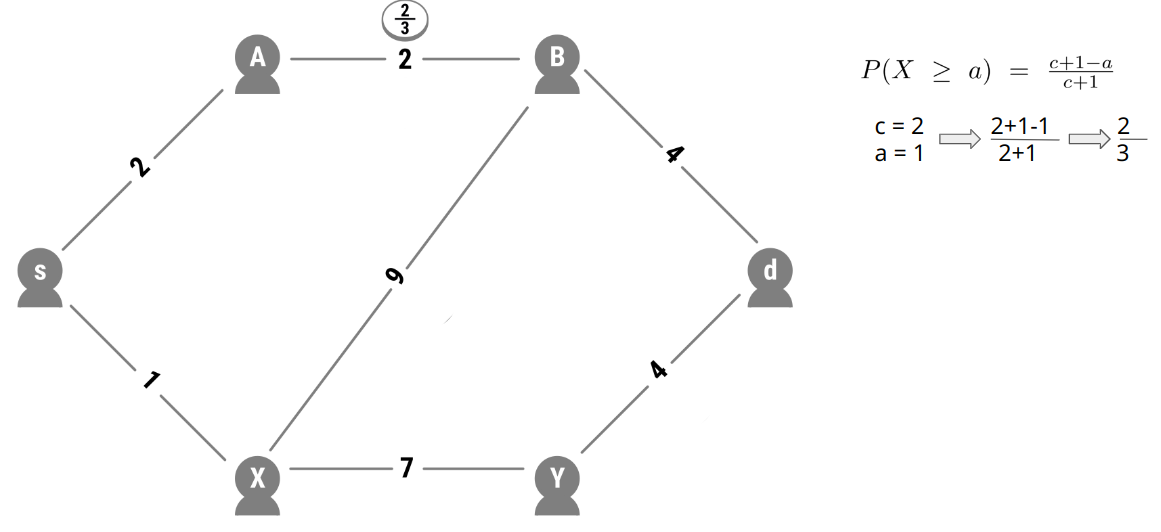
\includegraphics[width=0.6\columnwidth]{imgs/mincost_rene1.png}
  \end{center}
  \caption{Lightning Network Payment from A to B using channel success probability score.} 
  \label{fig:channel_success_prob_score}
\end{figure}


However, the paper shows also that with gossip data is difficult simulate 
a real envoirment, and this mean that the model described do not take into 
count the how fast an capacity $c(u, v)$ arrive to zero, or if this is a 
common case.

\subsection{Jamming Attach on Lightning}

Uncertain channel balances problem described in the previous section 
is not the only reason why payments on the lightning network are unreliable.
Another well known problem on the Lightning Network is \emph{jamming attack},
it is a cheap denial-of-service (DoS) attack, where the goal of this DoS attack 
is to prevent payments, either routed through the victim or paying the victim. 
The effectiveness of jamming thus could be characterized by the reduction of 
payment success rate, applied to the victim or the entire Lightning Network.

The paper \cite{cryptoeprint:2022/1454} decribe an solution to this problem 
based on a \emph{reputation system} and \emph{up-front fee} that allows to make
the Jamming attach costly due to the up-front fee and difficult to do during the time 
due to the reputation system.
In addition, the paper define different kind of Jamming attach, divided in :

\begin{itemize}
    \item {\bf Slow Jamming}: The attacker make a payment with a very long timeout, 
        in this way all channel along the route has the balance locked;
    \item {\bf Fast Jamming}: The attacker try to mimic the onest payment, by sending
        a failed payment; Currently in the Lightning Network there is a similar operation
        that it is used to steal information from a channel called probing.
\end{itemize}

In order to mitigate slow and fast jamming the paper \cite{cryptoeprint:2022/1454}
propose a combination of two strategies, combined in the following way:

\begin{itemize}
    \item {\bf Up-front fee} paid to the downstream peer addresses quick jamming 
        by imposing a small cost on every payment;
    \item {\bf Local reputation} based on past behavior addresses slow jamming by 
        punishing peers who forward payments that take too long to resolve.
\end{itemize}

The solution proposed regarding the unconditional fee are realative simple to implements 
because required to a node to pay for an attempt also if this fails (if succided the up-front fee can 
be returned back), and the choise of the path is driven by the local reputation that 
score the channel based on the following information:

\begin{itemize}
    \item  $\gamma$ (seconds): the maximal resolution time to consider a payment honest;
    \item  $\gamma$  (seconds), T (seconds), A (satoshis per second): reputation update 
    parameters;
    \item  K (integer), L(satoshis): the high-risk quota of slots and liquidity.
\end{itemize}


Calculating the Reputation Scores works by considering two possible values
for reputation scores:  \emph{high}  and  \emph{low}. Initially, all peers 
receive a low score. A payment is deemed  honest  if it resolves within  
$\gamma$  seconds, otherwise, it is considered a jamm attach. 
A peer’s behavior is defined as  good  if it only offers honest payments 
for forwarding. Moreover, those payments must pay at least A satoshis 
per second in fees to the routing node. Reputation of a peer grows if it 
demonstrates good behavior for a long enough period.
